% \documentclass[twocolumn,a4paper]{ieicejsp}
\documentclass[10pt,a4j,twocolumn,oneside]{jsarticle}
\setlength{\textwidth}{24zw}
%余白の設定ここから
\setlength{\topmargin}{25mm}
\addtolength{\topmargin}{-1in}
\setlength{\oddsidemargin}{15mm}
\addtolength{\oddsidemargin}{-1.1in}
\setlength{\evensidemargin}{20mm}
\addtolength{\evensidemargin}{-1in}
\setlength{\textwidth}{182mm}
\setlength{\textheight}{265mm}
\setlength{\headsep}{0mm}
\setlength{\headheight}{0mm}
\setlength{\topskip}{0mm}
%余白の設定ここまで
%twocolumn(2列)の間の空白の大きさ設定
\columnsep=8mm
\setlength{\baselineskip}{16pt}
\setlength{\headsep}{-5mm}
\renewcommand{\baselinestretch}{0.85}
% 図と図の間のスペース
\setlength\floatsep{0truemm}
% 本文と図の間のスペース
\setlength\textfloatsep{0truemm}
% 本文中の図のスペース
\setlength\intextsep{0pt}
% 図とキャプションの間のスペース
\setlength\abovecaptionskip{0truemm}
\setlength{\leftmargini}{10pt} 
\makeatletter

 \renewcommand\@maketitle{%
  %\newpage\null
  \vspace{-13mm}%
  \begin{center}%
  \let\footnote\thanks
    %{\LARGE \@title \par}%
    {\Large {\bf \@title} \par}
    %\vskip 1.5em%
    \vskip 0.5em
    {\large
      \lineskip 0.5em%
      \begin{tabular}[t]{c}%
        {\bf \@author }
      \end{tabular}\par}%
    \vskip 1em%
    {\large \@date}%
  \end{center}%
  \par \vskip 0.5em
}

\renewcommand\maketitle{\par
  \begingroup
    \renewcommand\thefootnote{\@fnsymbol\c@footnote}%
    \def\@makefnmark{\rlap{\@textsuperscript{\normalfont\@thefnmark}}}%
    \long\def\@makefntext##1{\parindent 1em\noindent
            \hb@xt@1.8em{%
                \hss\@textsuperscript{\normalfont\@thefnmark}}##1}%
    \if@twocolumn
      \ifnum \col@number=\@ne
        \@maketitle
      \else
        \twocolumn[\@maketitle]%
      \fi
    \else
      \newpage
      \global\@topnum\z@   % Prevents figures from going at top of page.
      \@maketitle
    \fi
    \thispagestyle{myheadings}\@thanks
  \endgroup
  \setcounter{footnote}{0}%
  \global\let\thanks\relax
  \global\let\maketitle\relax
  \global\let\@maketitle\relax
  \global\let\@thanks\@empty
  \global\let\@author\@empty
  \global\let\@date\@empty
  \global\let\@title\@empty
  \global\let\@correspondence\@empty% added for manuscript.cls
  \global\let\@affiliation\@empty% added for manuscript.cls
  \global\let\title\relax
  \global\let\author\relax
  \global\let\date\relax
  \global\let\and\relax
  \global\let\correspondence\relax% added for manuscript.cls
  \global\let\affiliation\relax% added for manuscript.cls
}
\makeatletter

\makeatletter
% \def\section{\@startsection {section}{1}{\z@}{-2.5ex plus -1ex minus -.2ex}{2.5 ex plus .2ex}{\Large\bf}}
\def\section{\@startsection {section}{1}{\z@}{0ex plus -1ex minus -.2ex}{.5ex plus .2ex}{\Large\bf}}
\def\subsection{\@startsection {subsection}{1}{\z@}{-1.5ex plus -1ex minus -.2ex}{2.3 ex plus .2ex}{\Large\bf}}
\def\subsubsection{\@startsection {subsubsection}{1}{\z@}{-2.5ex plus -1ex minus -.2ex}{.3 ex plus .2ex}{\large \bf $\spadesuit$ }}
\makeatother

% 参考文献
\makeatletter
  \renewenvironment{thebibliography}[1]{%
    \global\let\presectionname\relax
    \global\let\postsectionname\relax
    \section*{\refname}\@mkboth{\refname}{\refname}%
    \list{\@biblabel{\@arabic\c@enumiv}}%
          {\settowidth\labelwidth{\@biblabel{#1}}%
          \leftmargin\labelwidth
          \advance\leftmargin\labelsep
          % 文字サイズ?
          \setlength\baselineskip{9pt}
          % アイテム間のマージン
          \setlength\itemsep{.3zh}
          \@openbib@code
          \usecounter{enumiv}%
          \let\p@enumiv\@empty
          \renewcommand\theenumiv{\@arabic\c@enumiv}}%
    \sloppy
    \clubpenalty4000
    \@clubpenalty\clubpenalty
    \widowpenalty4000%
    \sfcode`\.\@m}
    {\def\@noitemerr
      {\@latex@warning{Empty `thebibliography' environment}}%
    \endlist}
\makeatother

\makeatletter
\def\@listi{\leftmargin\leftmargini
\parsep \z@
\topsep 0\baselineskip \@plus 0.1\baselineskip \@minus 0.1\baselineskip
\itemsep \z@ \relax}
\let\@listI\@listi
\makeatother


\usepackage{newenum}
%\usepackage{epsfig}
%\usepackage{ascmac}
%\usepackage{amsmath}
%\usepackage{nccmath}
\usepackage{listings}
\usepackage{comment}
\usepackage{newtxtext}
\usepackage{textcomp}
%\usepackage{newtxmath}
%\usepackage{svg}
\usepackage[dvipdfmx]{graphicx}
\usepackage{fancyvrb}
% \usepackage{multicol}
\usepackage{url}
\usepackage[subrefformat=parens]{subcaption}
\pagestyle{empty}

% subsubsectionを再定義する.
\makeatletter
\renewcommand{\subsubsection}{\@startsection{subsubsection}{3}{\z@}%
  {1.0\Cvs \@plus.5\Cvs \@minus.2\Cvs}%
  {0.5\Cvs \@plus.3\Cvs}%
  {\reset@font\normalsize\bfseries}}
\makeatother

%論文のタイトル等記述
%ここから
\title{
  {\bf
  非日照時間の水位推定のためのノイズ除去手法の検討
}}
\author{佐々木 七海 (指導教員 島 和之 准教授)}
\date{}           %日付は不要なので書かないこと
%ここまで

\setlength{\baselineskip}{16pt}
%\setlength{\headsep}{-5mm}
\renewcommand{\baselinestretch}{0.95}

\begin{document}

%諸事情により, maketitleコマンドを変更してます
%の部分は変更しないこと
%\input{newtitle}
%ここまで


\maketitle
\thispagestyle{empty}

%ここから本文書き始め

\section{はじめに}
%\vspace{-3mm}

土砂災害は日本全国で多発しており、日本全国の直近10年間の年間平均で1400件以上発生している。
  % また、集中豪雨が発生した2018年には国内で3500件近くの土砂災害が発生したことが報じられている。
  % (こういった背景として、日本には中小河川が多く存在し、流量面積が小さいため、豪雨に伴い、
  % 土砂災害の一つである土石流が発生しやすいということが挙げられる。)
% 土砂災害の一つである土石流には「河川の水位が急激に減少する」という前兆現象があることが知られ
% ている。
  % これは、土石流の発生前に河川上流で土砂や倒木が河川の流れを堰き止め、河川下流に向かう水流が急
  % 激に減少することによって生じる現象である。
本研究では、河川監視カメラから得られる画像から水位の推定を行うことで、「降雨が続いている
にもかかわらず、河川の水位が急激に減少する」という土石流の前兆現象を捉えて土石流発生の事前予
測を行うための水位推定を可能にすることを目指す。
先行研究では、3日間に撮影された河川監視カメラ画像のうち、
  % (7:00~18:00までの)
日照時間帯において河川の水位を推定し、量水標から測定した真値と比較してその精度評価を行った。こ
こでは、3日間各日の
% 0:00~日の出と日の入り以降の
非日照時間においては研究の対象外とされたため、未検証のままである。
実際の土石流事前予測を行うには、深夜や早朝の時間帯においても精度を大きく下
げることなく推定を可能にすることが必須であると考える。しかしながら、深夜の監視カメラ画像は全体
的に暗く降雨によるノイズや異物がより顕著に現れ、水位推定の障害となっている。
本研究では非日照時間のノイズを含む監視カメラ画像に焦点を当て、高い精度で水位の推定を行うための
ノイズ除去方法を検討する。
\section{先行研究}
%\vspace{-3mm}
本研究では、先行研究で提案された推定手法によってノイズ除去後の精度評価のための水位推定を行う。
以下では先行研究の手法を記述する。
\subsection{累積差分画像の生成}
先行研究の手法では、差分による水面変化の抽出と差分画像の累積を行い、累積差分画像を生成する。
この累積差分画像から水面領域、水位の推定を行う。
具体的には、河川の監視カメラで撮影される時系列画像の隣接時刻間で差分を行い、絶対差を
求めることで水面の時系列変化を抽出する。これにより、時々刻々と変化する水の流れや光による反射、
屈折等による水面変化のみが抽出される。これを各時刻間で行い、水面変化を抽出する。さらに差分に
より求めた絶対差を一定時間分累積する。この累積差分画像により、水面全体をとらえることが可能に
なる。得られた累積差分画像に対し、深層学習であるDeepLabV3+を適用し、水面領域の推定を行う。こ
の水面推定領域の面積割合位から水位に変換する変換式を用いることにより、水位変動推定精度を調べる。
用いる変換式は量水標から読み取れる水位の真値と水面の正解領域を記した画像の関係を調べ立式を行う。

% \begin{figure}[t]
%   \begin{minipage}[b]{0.49\linewidth}
%     \centering
%     %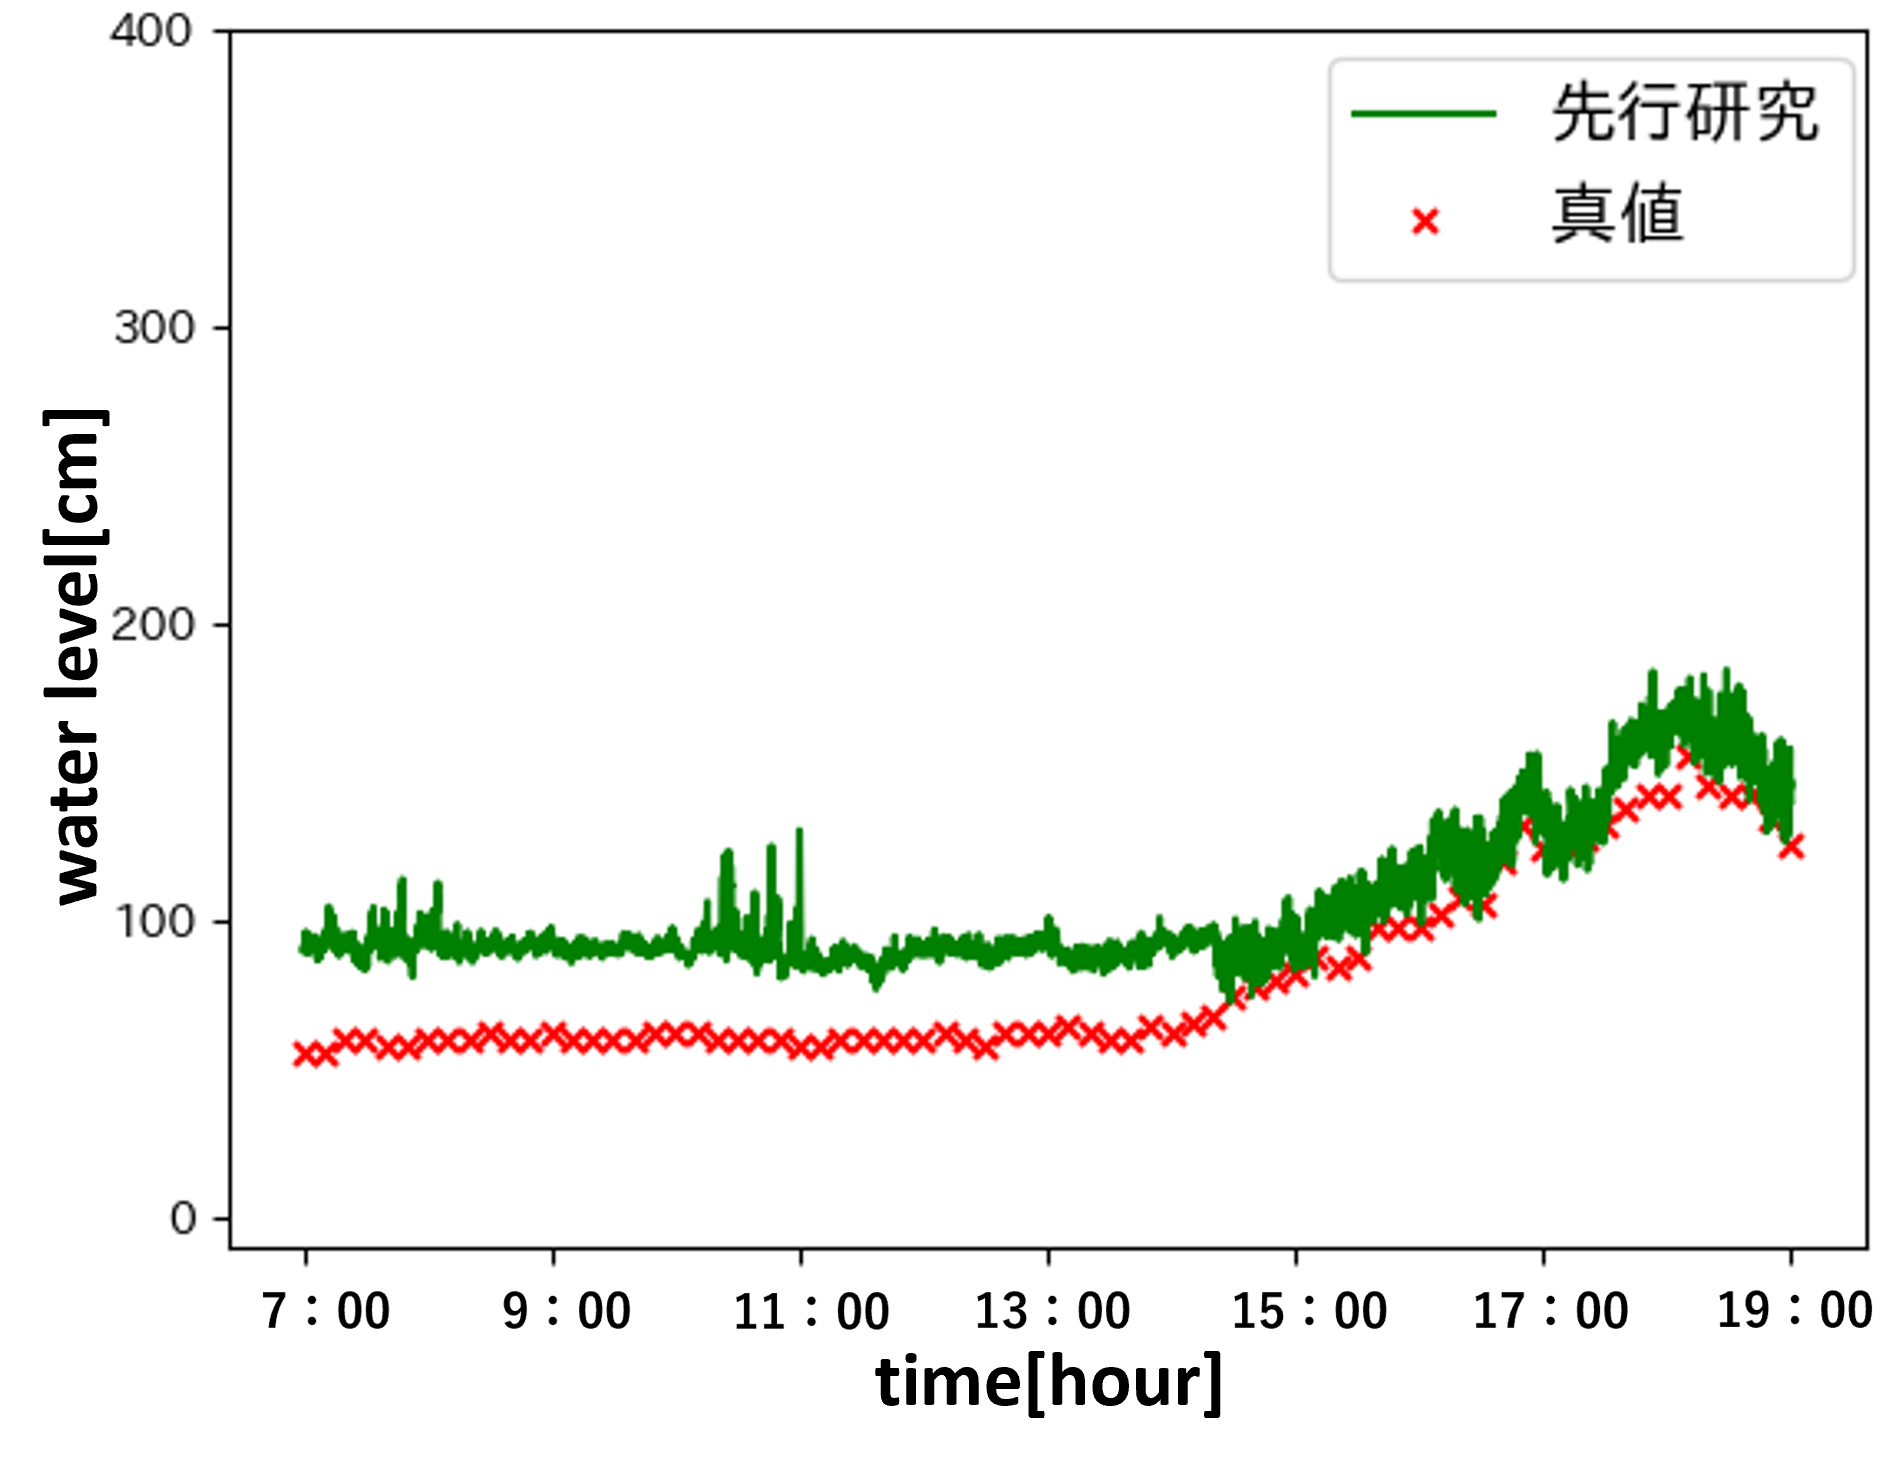
\includegraphics[keepaspectratio, scale=0.3]{./figs/20180706_watanabe_re.png}
%     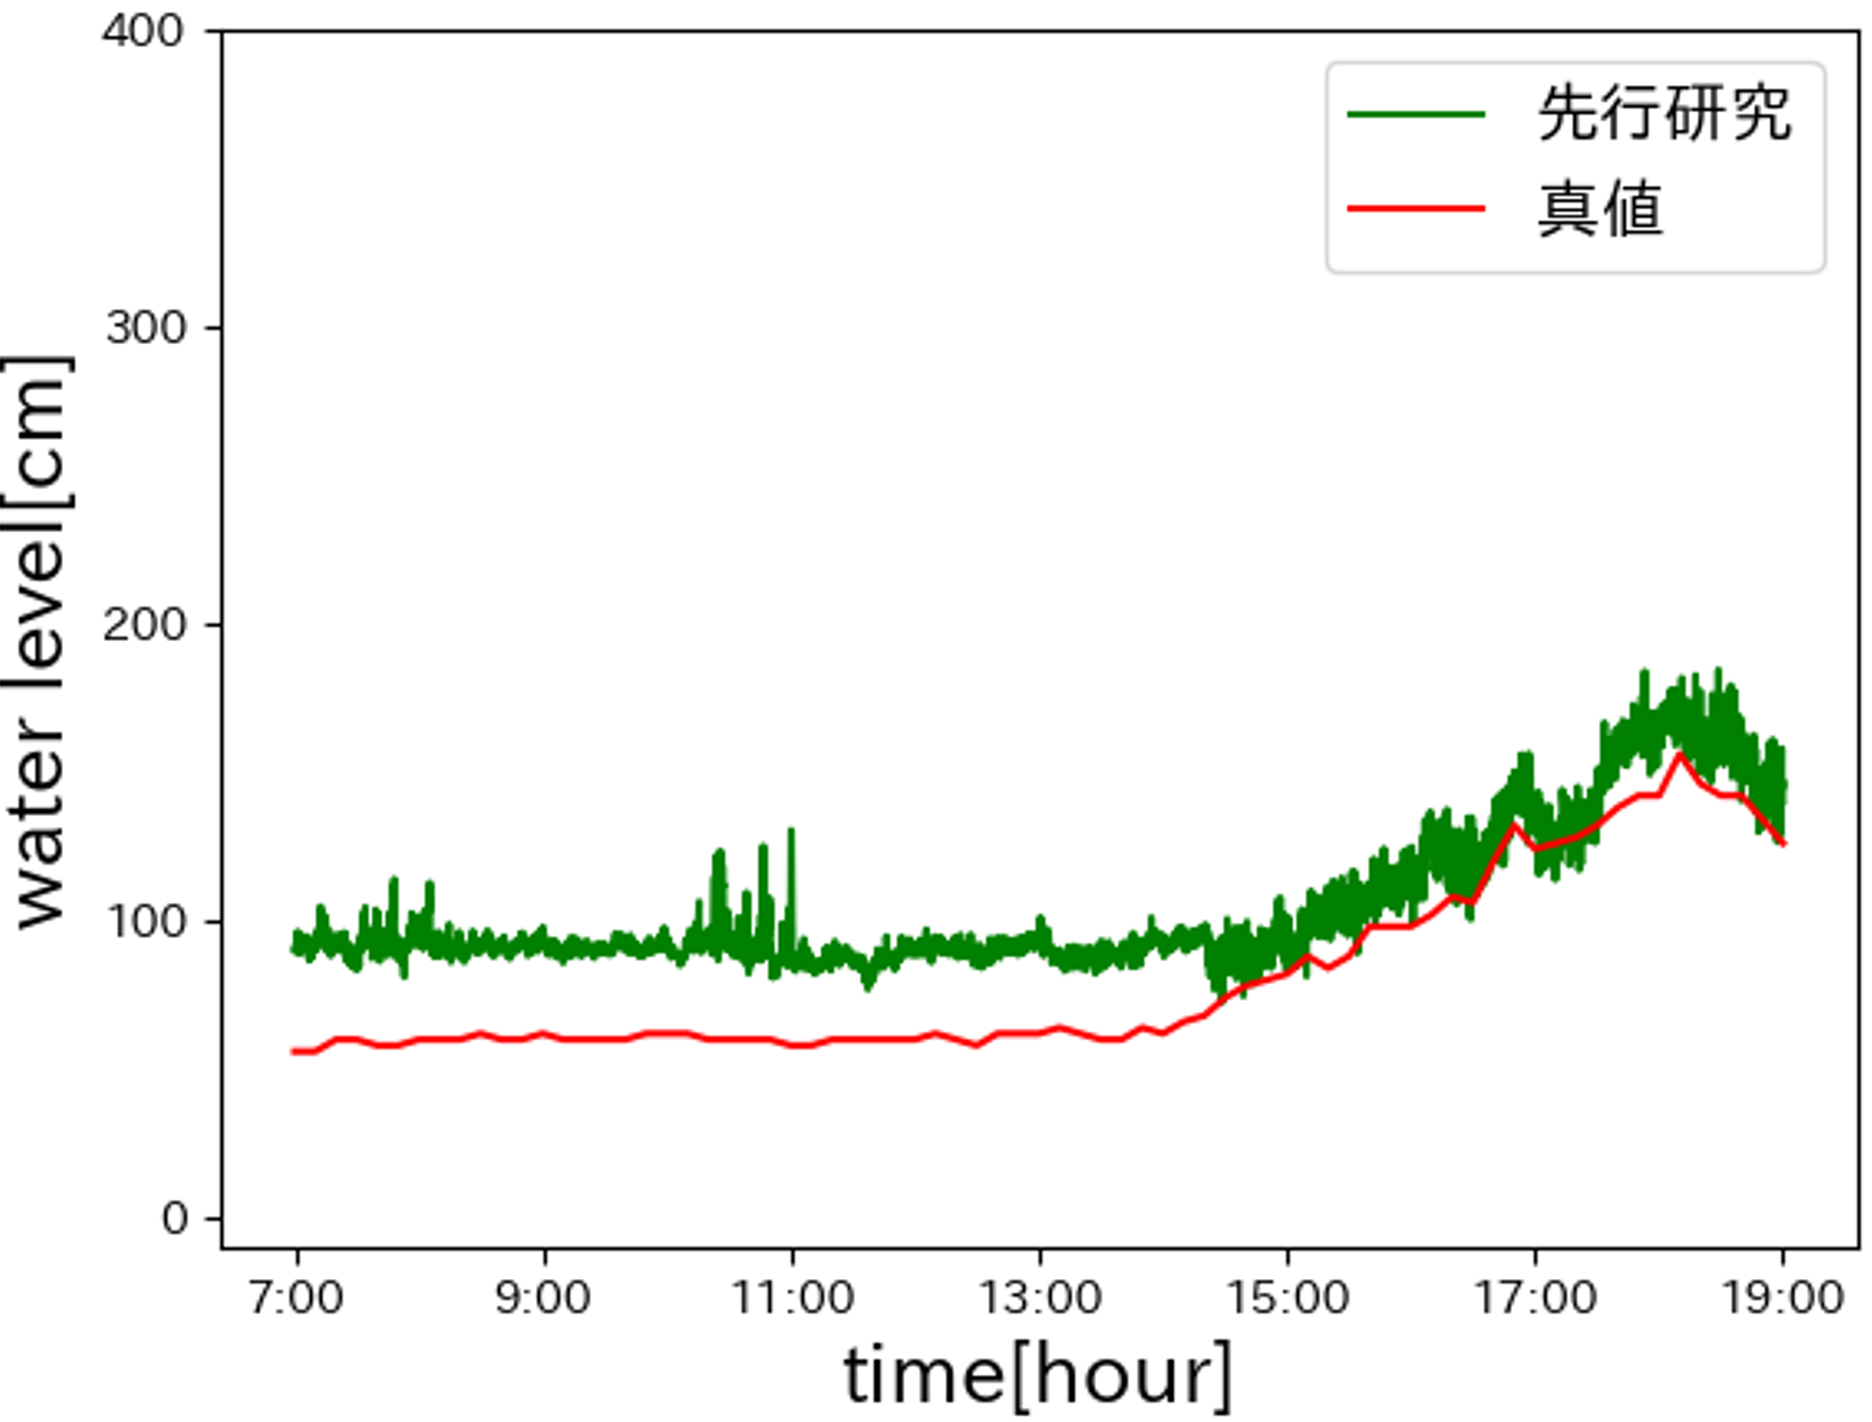
\includegraphics[keepaspectratio, scale=0.3]{./result/watanabe20180706.png}
%     \subcaption{先行研究}
%   \end{minipage}
%   \begin{minipage}[b]{0.49\linewidth}
%     \centering
%     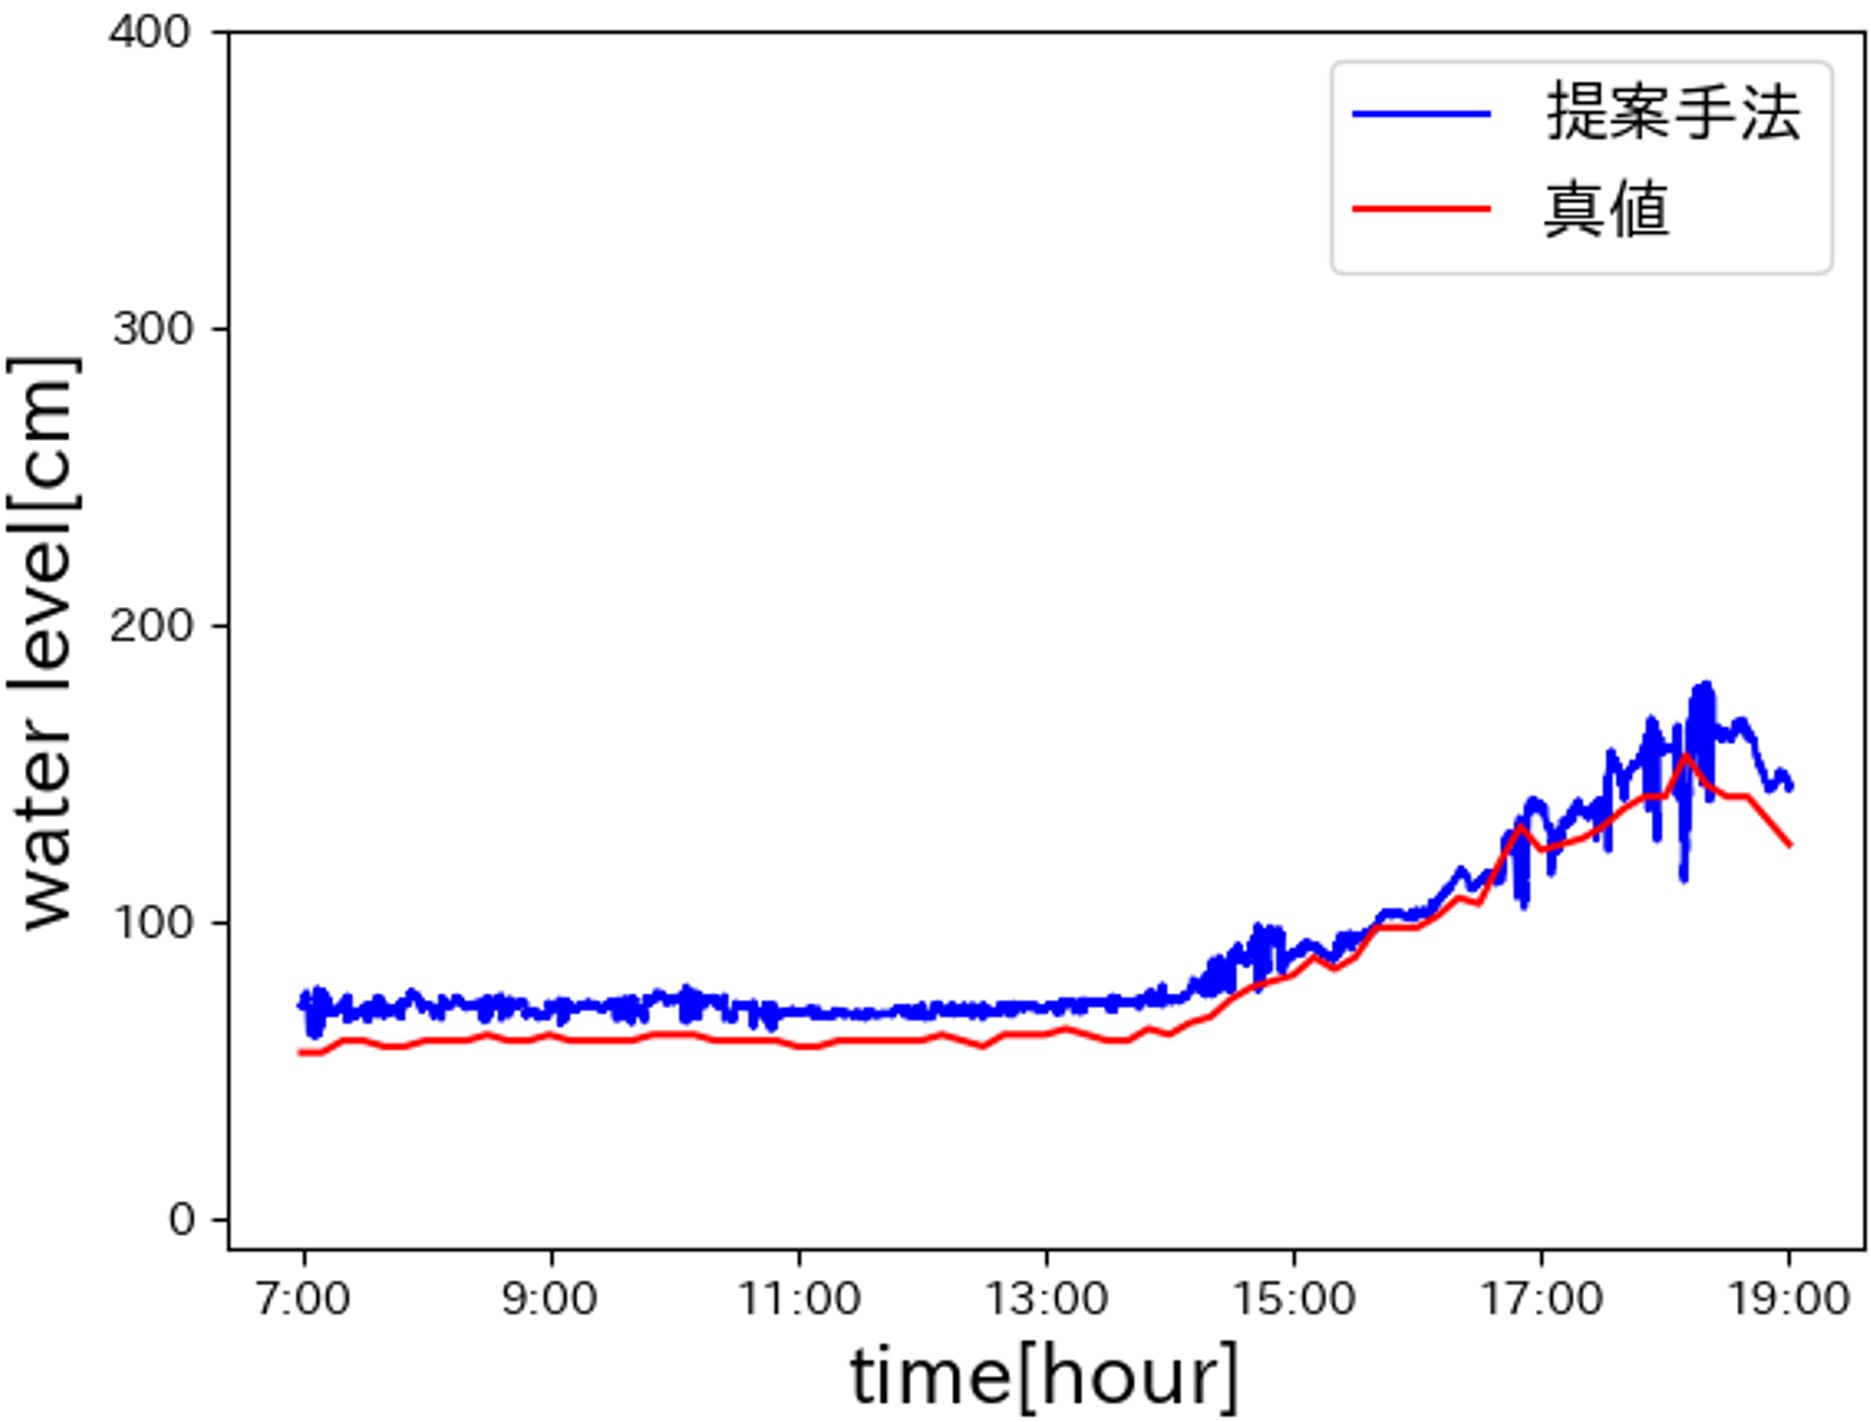
\includegraphics[keepaspectratio, scale=0.3]{./result/hirai20180706.png}
%     \subcaption{提案手法}
%   \end{minipage}
%   \caption{2018年7月6日の水位変動推定結果}
%   \label{fig:image2}
% \end{figure}

% \begin{figure}[t]
%   \begin{minipage}[b]{0.49\linewidth}
%     \centering
%     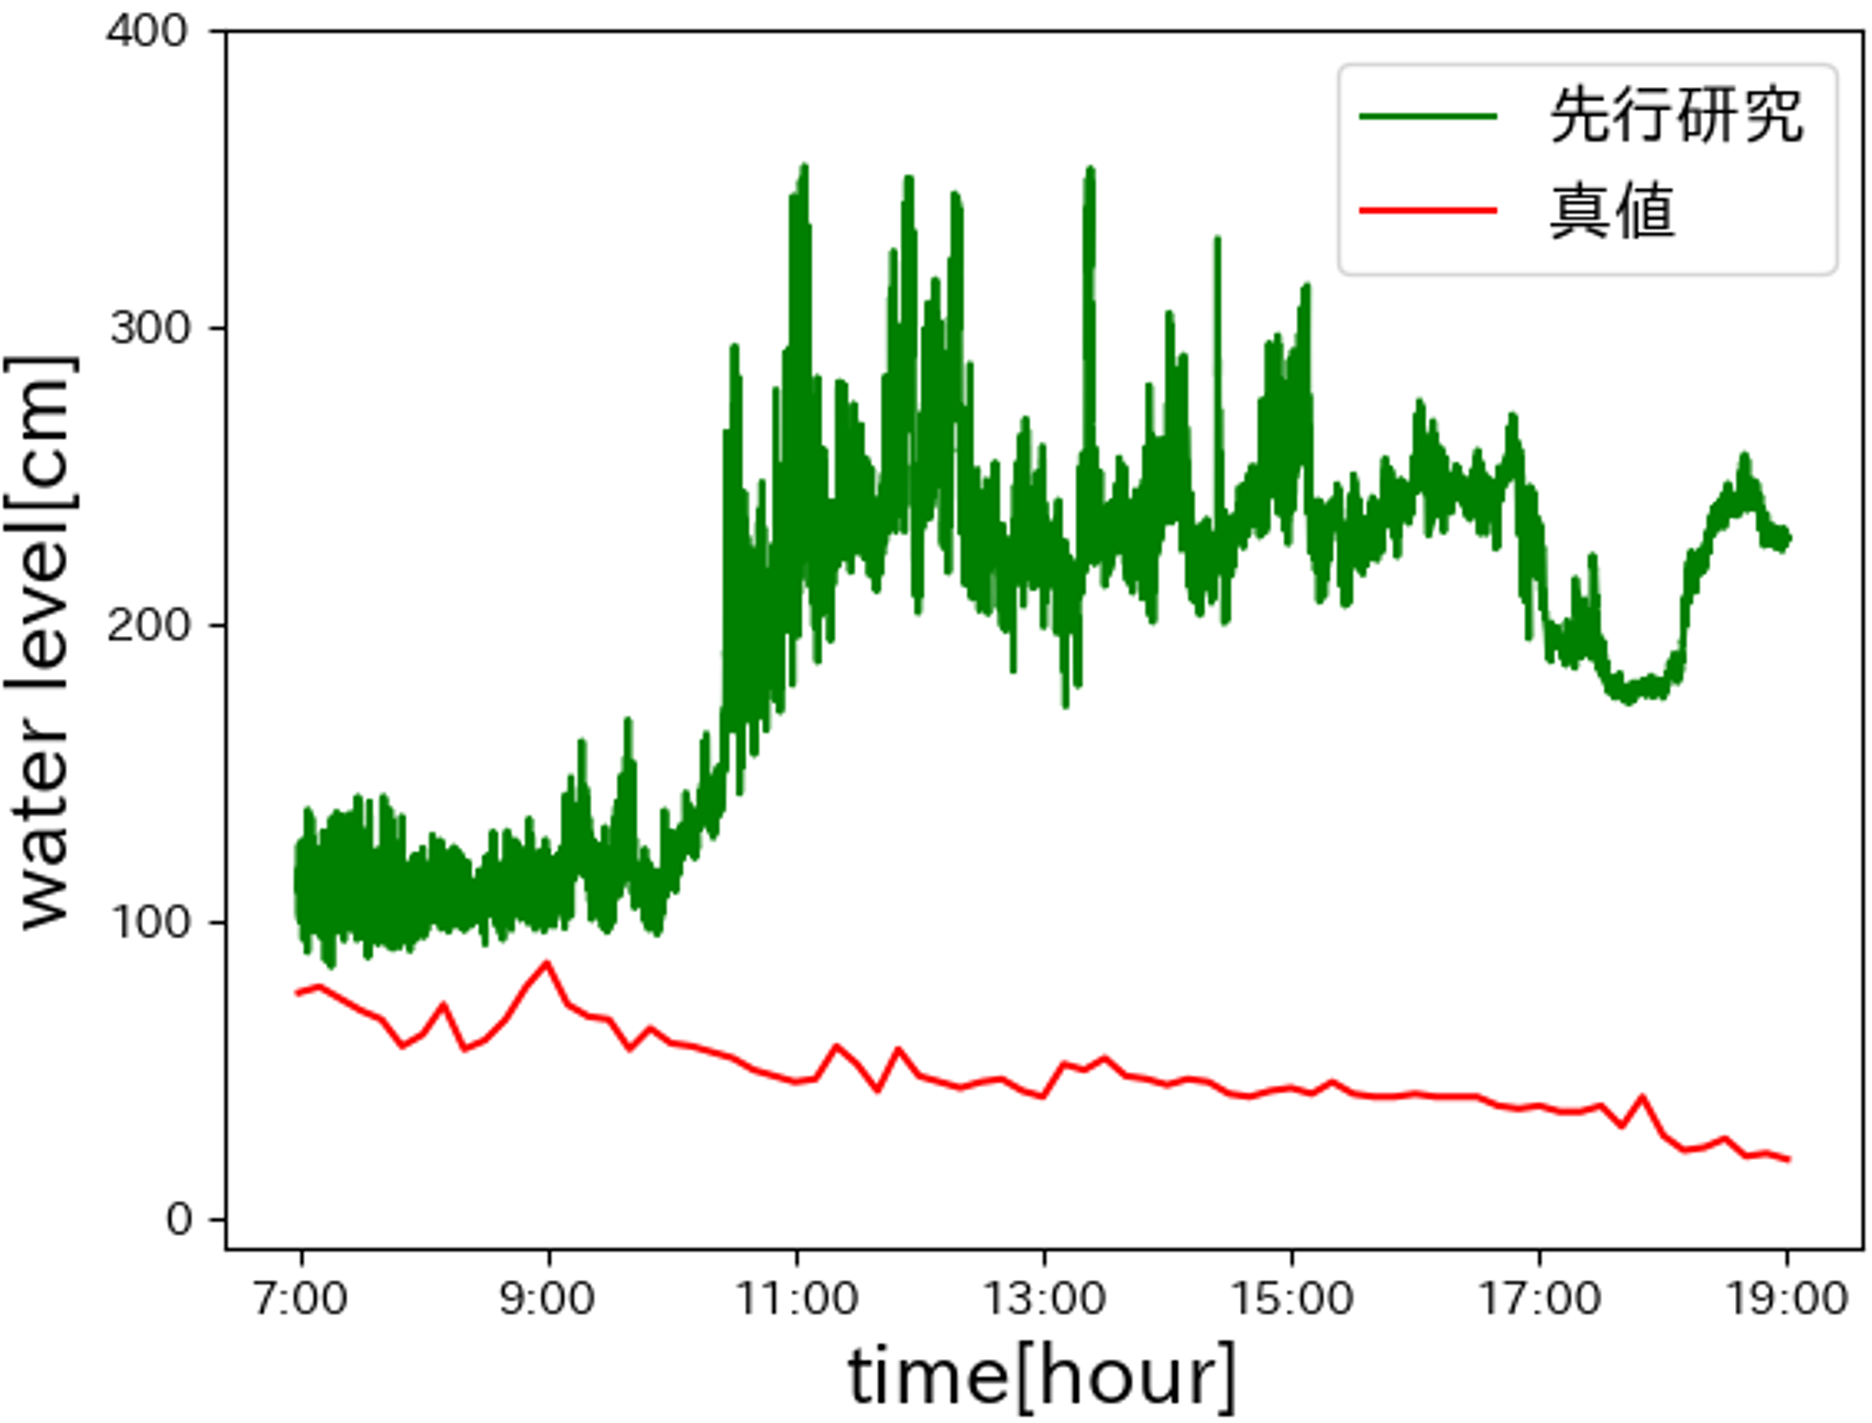
\includegraphics[keepaspectratio, scale=0.3]{./result/watanabe20180707.png}
%     \subcaption{先行研究}
%   \end{minipage}
%   \begin{minipage}[b]{0.49\linewidth}
%     \centering
%     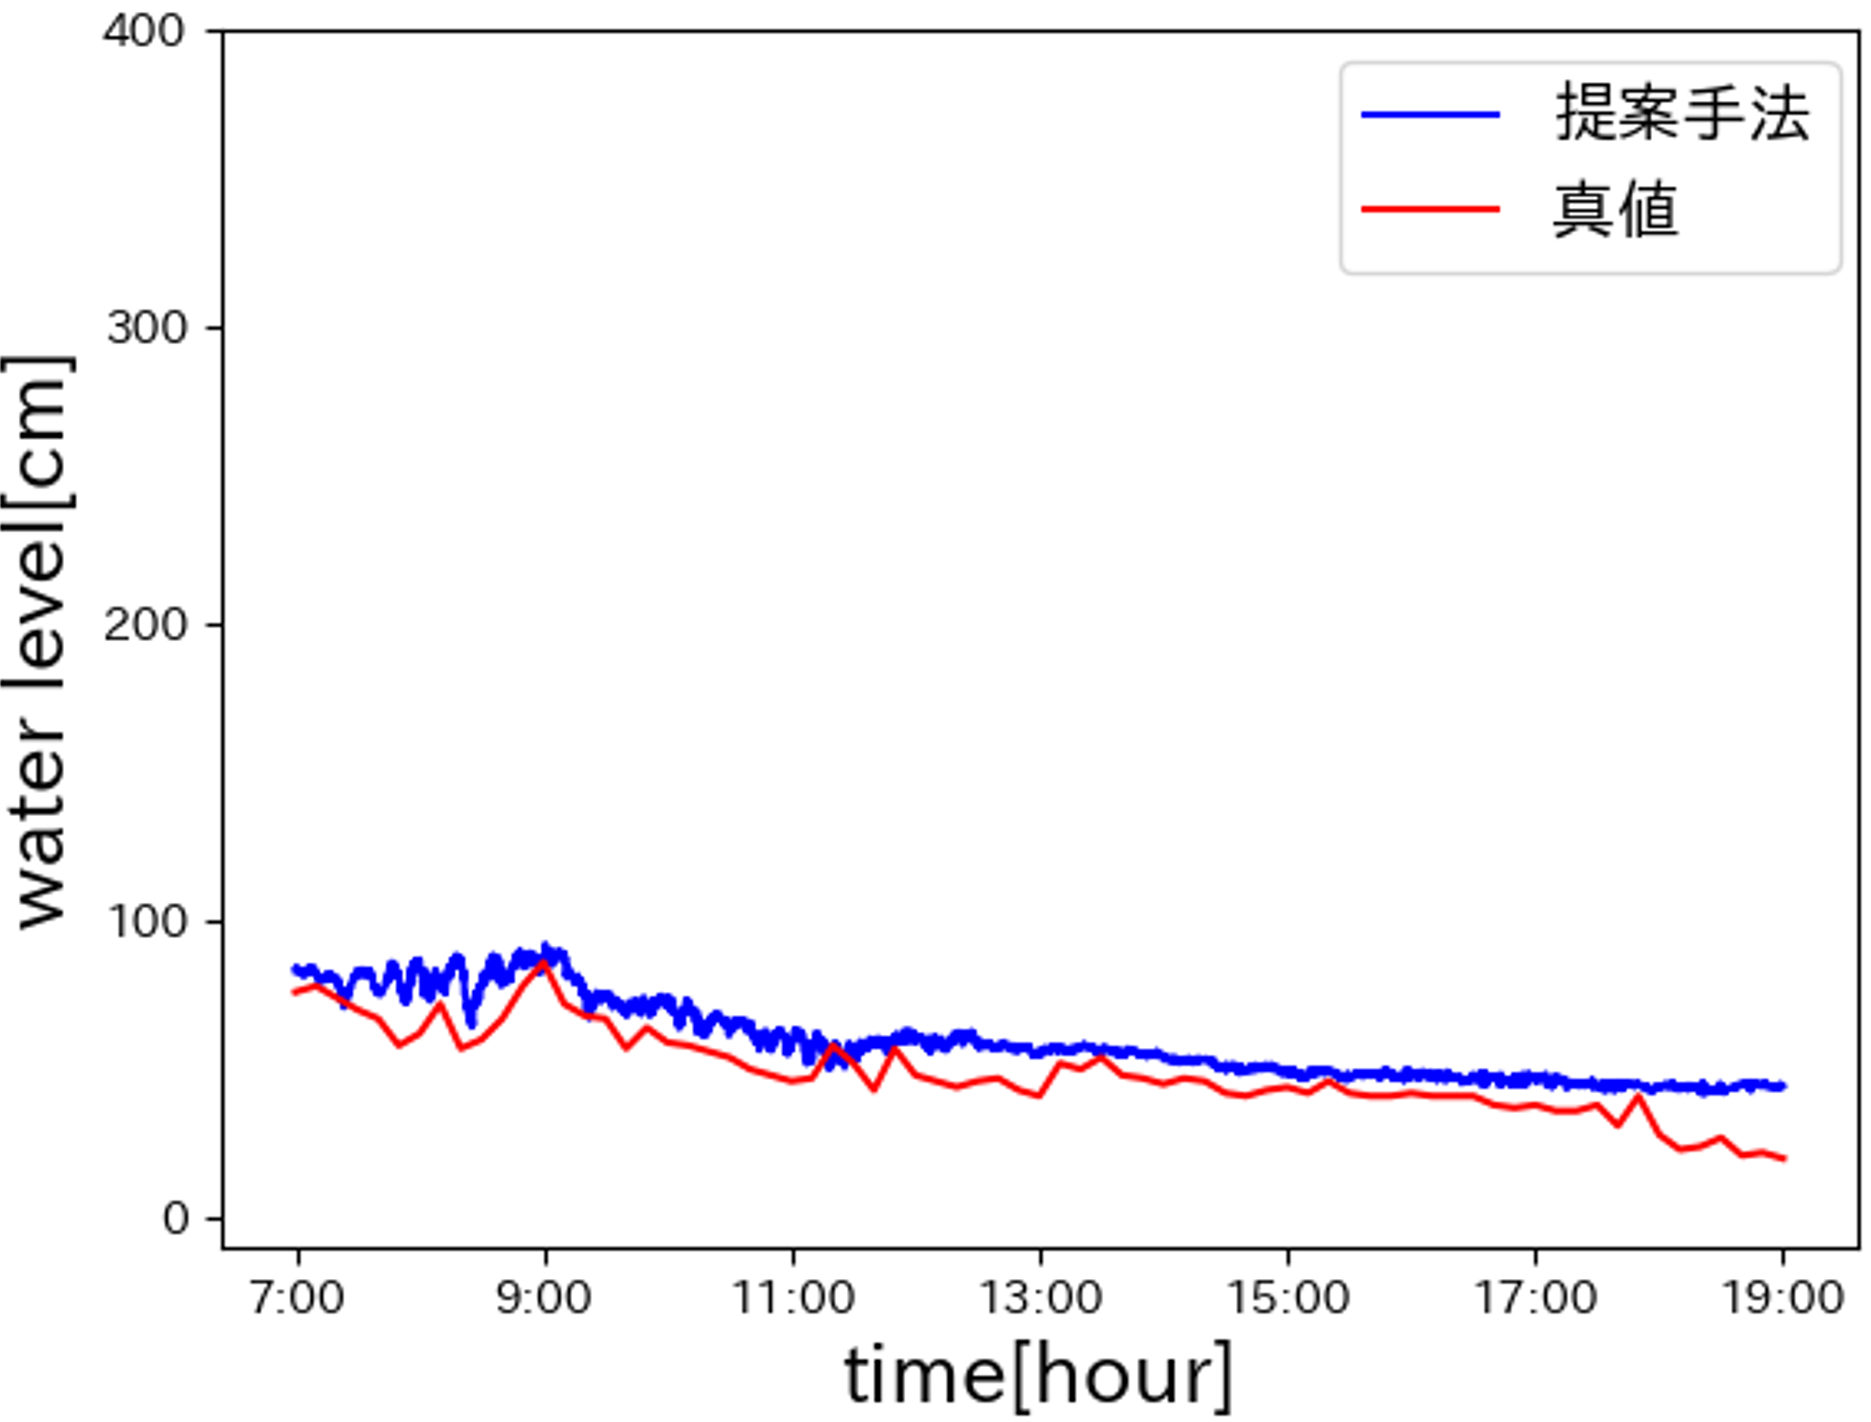
\includegraphics[keepaspectratio, scale=0.3]{./result/hirai20180707.png}
%     \subcaption{提案手法}
%   \end{minipage}
%   \caption{2018年7月7日の水位変動推定結果}
%   \label{fig:image3}
% \end{figure}

\section{提案手法}
深夜の監視カメラ画像においては、全体の輝度値が低く雨粒や降雨の光の反射が顕著に現れる。
これらが先行研究の手法において深夜での水位推定の精度を低下させる要因となっている(図)。
(図:ノイズのある深夜の監視カメラ画像の例)
(図:未処理の状態で水面領域を推定した結果の失敗例)
したがって、本研究ではこれらのノイズの範囲を検出可能にし、さらに検出した範囲に対して
ノイズを除去する手法を検討する。さらにその効果を調べるため、提案手法に対し先行研究の手
法に基づいて水位推定を行い精度評価を行う。
  \subsection{ノイズ部分の検出}
    % \subsubsection{Hough変換による検出}
    \subsubsection{輝度値の閾値を利用}
    カメラ画像をグレースケールに変換した後、ヒストグラムを作成し各画素に格納された輝度
    値のうちノイズ部分の分布する輝度値を閾値として設定する。この閾値を超えた輝度値をも
    つ画素部分をノイズ部分と定める。
  \subsection{ノイズ除去手法}
    % \subsubsection{モルフォロジー変換によるノイズ除去}
    \subsubsection{輝度の閾値によるノイズ除去} 
    河川画像の水位推定においては、水面と背景の2つの領域の境目を求めることが肝心である。
    この領域の境目の特徴をノイズ除去後も保つために画像の画素値配列の各行ごとに、輝度値
    の平均値を求める。閾値により定めたノイズ部分の各画素に対し、各行の輝度値の平均値に
    置き換えることにより、水平方向の特性を保ったままノイズ部分による影響を低減する。

%\vspace{-5mm}
% 本研究で使用する画像は,本学情報工学科モニタリングネットワーク研究室で
% 運用されている広島市安佐北区三入地区桐原川の監視カメラから得られる画像を用いる.
% 得られる画像のうち,2018年7月5日,2018年7月6日,2018年7月7日の
% 7:00から19:00までの12時間分のデータを用いて実験を行う.
% また,この監視カメラは動かないよう固定されており,5秒間隔で河川画像を取得している.
% そのため,隣接時刻間で差分を行う際5秒間で観測される水面変化を抽出し,
% 累積時間$T_{past}$は1,2,3,4,5分としてそれぞれで水面領域と水位変動の推定を行う.
% 累積差分画像から水面領域を推定する3つの方法の1つである大津の2値化を適用した結果と
% 先行研究\cite{Watanabe.K}の結果と比較を行った.
% 比較する評価指標として推定された水面領域を水位に変換し
% 水位の真値との二乗平均平方根誤差(RMSE)を用いる.
% ここでは,累積時間$T_{past}$を5分とした累積画像を用いて
% 水位の上昇が見られる2018年7月6日の水位変動推定結果を図\ref{fig:image2}に,
% 水位の減少が見られる2018年7月7日の水位変動推定結果を図\ref{fig:image3}に示す.
% 真値との誤差(RMSE)は,
% 2018年7月6日では先行研究で26.09[cm],提案手法で11.55[cm]となり,
% 2018年7月7日では先行研究で163.44[cm],提案手法で11.74[cm]となった.

% \begin{table}[t]
%   \centering
%   \caption{先行研究,提案手法の推定値と真値の誤差(RMSE)[cm]}  
%   \begin{tabular}{|r||r|r|} \hline 
%    &  先行手法  &  提案手法  \\ \hline \hline
%    2018年7月6日 & 26.09 & 9.63 \\ \hline
%    2018年7月7日 & 163.53 & 8.64 \\ \hline   
%   \end{tabular}
%   \label{t_2}
%   \vspace{3mm}
% \end{table}
\section{実験}
対象画像には同日の非日照時間における雨粒や降雨によるノイズを含む時系列画像3394枚を
用いる。
各画像ごとのノイズ部分を含む画素値配列の行ごとの平均値をとり、平均値を超える画素を
ノイズ部分として処理の対象とする。
次に処理の対象として検出された画素に対し、ノイズ部分を含まない画素値配列の行ごとの
平均値に変換する処理を行う。これにより、ノイズ部分のみ輝度値が大きいことによる推定
精度の低下を防ぐ。
\section{結果}
(表にする)
処理前の推定結果:RMSE=20.94[cm]
処理後の推定結果:RMSE=8.991[cm]

\section{まとめ}
本研究では、非日照時間の河川監視カメラにおけるノイズ除去の手法を検討し、推定精度の
変化を調べた。提案手法では画像の輝度値の行ごとの平均値を用いてノイズ部分の検出と処
理を行うことで、水平方向の特徴を保ったまま輝度値の大きいノイズによる推定精度の低下
の阻止を図った。
今後の課題としてはより定量的かつ汎用的な閾値の設定方法を調べることや、ノイズ部分と
して検出された画素に対しより効果的にノイズによる精度低下を改善する方法について調べ
ることが考えられる。

% 図\ref{fig:image2}から先行研究,提案手法ともに正確に推定できているが,
% 提案手法ではより真値と誤差の小さい水位推定ができていることが確認できる.
% 図\ref{fig:image3}では先行研究は推定誤差が大きいが,
% 提案手法では真値と同様の水位変動が見られる.
% いずれのデータでも先行研究よりも小さい誤差の結果が得られたため,
% 水位変動の推定精度は累積画像を用いることによって大きく精度が向上したと考えられる.
% 特に2018年7月7日のデータでは同じ壁面でも場所によって輝度値が異なり,
% 先行研究で使用した学習モデルのデータに含まれていないため推定精度が低下している.
% 一方,累積差分画像では隣接時刻間での水面変化を用いているため影響を受けないことが
% 推定精度の向上に繋がったと考えられる.

% \section{まとめと今後の課題}

% 本研究では,河川の水面の時系列変化を用いることによって
% 水位変動の推定を行った.
% 水面変化を隣接時刻間の差分で求め,それを累積した累積差分画像から
% 水面領域の推定,推定された水面面積を水位に変換した水位変動の推定を行った.
% 先行研究の推定値と比較を行い,
% 提案手法の有効性を確認することができた.
% このことから,提案手法によって水位から分かる災害の前兆現象を
% より高精度に推定できることが可能であると考えられる.

% 今後の課題として夜間や他地点の観測データなどの適用範囲の拡大を行い,
% 汎用性の拡大を目指したい.
% 本研究では1地点の観測データで監視カメラが鮮明に撮影できる時間帯の画像を使用しているため,
% 前述したデータにも適用できるよう検討する必要がある.
% また,天候や個々の地形の特徴などの因子を考慮することでより迅速な災害予測・検知が期待される.
% \section*{発表論文}
% \noindent\underline{平井孝明}, 島和之:河川の連続画像の差分に基づく水位変動の推定,2023年電子情報通信学会 総合大会,2023年3月.
% \noindent\underline{平井孝明}, 島和之:河川の累積差分画像に基づく水位変動の推定,第74回電気・情報関連学会中国支部連合大会,2023年10月.

%本文ここまで

%参考文献はこのようにすると,一回り小さい文字で書いてくれる
% \small
% \bibliography{references}

\begin{thebibliography}{9}

% \bibitem{katsuyou}
% 国土交通省水管理・国土保全局砂防部 : 
% 「土砂災害警戒避難に関わる前兆現象情報の活用のあり方について」, 
% \url{http://www.mlit.go.jp/common/001021004.pdf} (2006-3). 

% \bibitem{Watanabe.K}
% 渡邊 康平, 島 和之 : 
% 「画像切抜と深層学習を用いた水位変化の推定」,
% 2022 年度 (第 73 回) 電気・情報関連学会中国支部連合大会 (2022-10).

% \bibitem{Nur}
% Nur, A.M., Ahmad, F.A., Siti, K.B., Muhammad, R.M., Ana, M. : 
% ``Deep Learning Semantic Segmentation for Water Level Estimation Using Surveillance Camera,''
% Applied. Science. 2021,vol.11, No.9691 (2021-10).	

% \bibitem{DeeplabV3+}
% Chen, L.-C., Zhu, Y., Papandreou, G., Schroff, F., Adam, H. : 
% ``Encoder-Decoder with Atrous Separable Convolution for Semantic Image Segmentation,''
% Proceedings of the European Conference on Computer Vision(ECCV), pp.801-818 (2018).

% \bibitem{Outsu}
% Nobuyuki, O. :
% ``A threshold selection method from gray level histograms,''
% IEEE Trans. Syst. Man Cybern., vol.9, no.1, pp.62-66, 1979.

\end{thebibliography}

\end{document}
